\documentclass[english]{tktltiki}
\usepackage[pdftex]{graphicx}
\usepackage{subfigure}
\usepackage{url}
\begin{document}
%\doublespacing
%\singlespacing
\onehalfspacing

\title{Digital Humanities Hackathon 2017 in Helsinki  \\ 
	Experiences by a computer scientist}
\author{P�ter Ivanics}
\date{\today}

\maketitle

\numberofpagesinformation{\numberofpages\ pages + \numberofappendixpages\ appendices}

\mytableofcontents

\section{Introduction}
	Digital humanities is an emerging field of science, which applies modern data processing methods to answer social science and humanities oriented research questions. This way scholars can study their own field from a new angle via the application of methods traditionally used in computer science. As a result, humanist researchers do not necessarily have to closely read historical text, but can take a look at the data from a new point of view, from a different angle. As the amount of such text has grown large along the centuries, manual labour has proven not to be sufficient to process all of the material and there is need for the assistance of computational methods. 
	
	I was lucky enough to participate in the Digital Humanities Hackathon organized by University of Helsinki and Aalto University in this year. During an intensive week of collaboration May 2017, historians, linguists, psychologists and computer scientists were brought together under the hood of this event. This post shortly summarizes my own experiences as a member of one of the interdisciplinary groups working on the digitized archive of Finnish newspapers from the 19th century. 

\section{Discussion}
	The group \textit{Categories, norms and genres - critical reading in numbers} consisted of two historians, two computer scientists, two linguists and a philosopher. On top of that, the composition of the group was not only interdisciplinary but also intercultural, because members were coming from four different countries. 
	
	We were given access to the Digital Newspaper Archive \footnote{\url{http://digi.kansalliskirjasto.fi/?language=en}}, which contains huge amount of digitized material from newspapers and journals published in Finland. Some of the data is freely available for anybody to process, but a considerable amount is copyrighted (Figure \ref{data_in_digi}). 
	
	\begin{figure}[h] 
		\begin{center}
			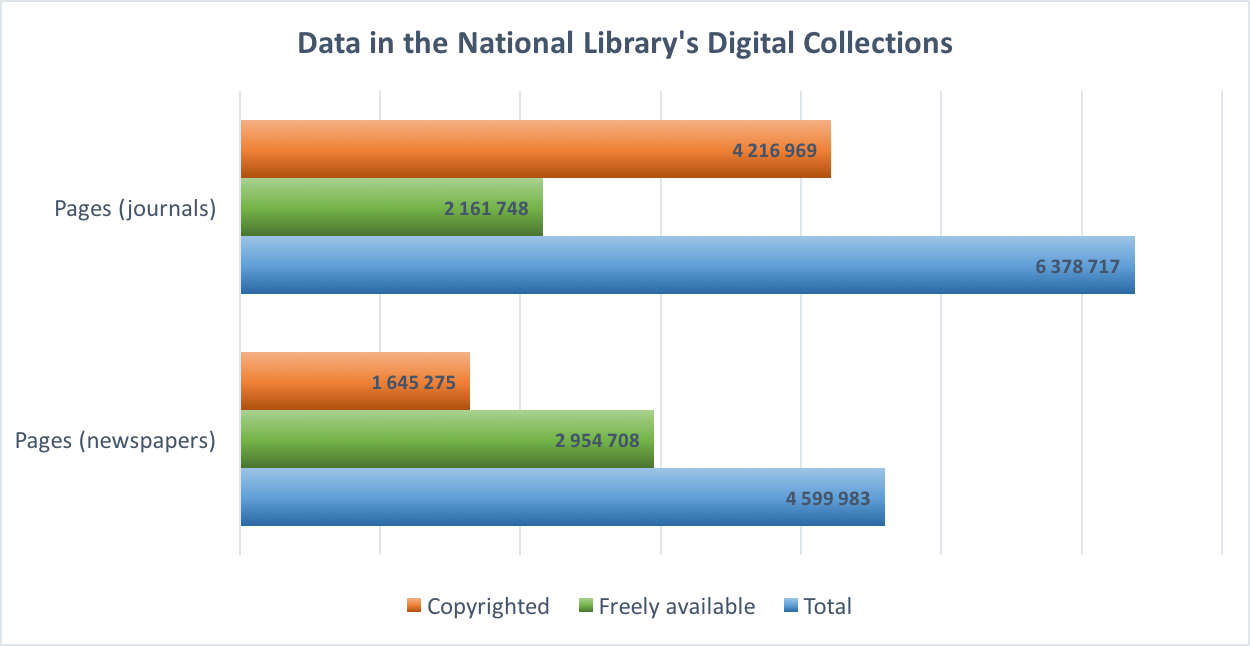
\includegraphics[width=0.9\textwidth]{images/data_in_digi.png}
			\caption{The distribution of the data in the digital archive of the Finnish National Library.}
			\label{data_in_digi}
		\end{center}
	\end{figure}	

\section{Conclusion}


\nocite{*}

\lastpage

\end{document}


